\documentclass[a4paper,12pt, oneside]{book}

% \usepackage{fullpage}
\usepackage[italian]{babel}
\usepackage[utf8]{inputenc}
\usepackage{amssymb}
\usepackage{amsthm}
\usepackage{graphics}
\usepackage{amsfonts}
\usepackage{listings}
\usepackage{amsmath}
\usepackage{amstext}
\usepackage{engrec}
\usepackage{rotating}
\usepackage[safe,extra]{tipa}
\usepackage{showkeys}
\usepackage{multirow}
\usepackage{hyperref}
\usepackage{microtype}
\usepackage{enumerate}
\usepackage{braket}
\usepackage{marginnote}
\usepackage{pgfplots}
\usepackage{cancel}
\usepackage{polynom}
\usepackage{booktabs}
\usepackage{enumitem}
\usepackage{framed}
\usepackage{algorithm}
\usepackage{algpseudocode}
\usepackage{pdfpages}
\usepackage{pgfplots}
\usepackage[cache=false]{minted}

\usepackage{tikz}\usetikzlibrary{er}\tikzset{multi  attribute /.style={attribute ,double  distance =1.5pt}}\tikzset{derived  attribute /.style={attribute ,dashed}}\tikzset{total /.style={double  distance =1.5pt}}\tikzset{every  entity /.style={draw=orange , fill=orange!20}}\tikzset{every  attribute /.style={draw=MediumPurple1, fill=MediumPurple1!20}}\tikzset{every  relationship /.style={draw=Chartreuse2, fill=Chartreuse2!20}}\newcommand{\key}[1]{\underline{#1}}

\usepackage{fancyhdr}
\pagestyle{fancy}
\fancyhead[LE,RO]{\slshape \rightmark}
\fancyhead[LO,RE]{\slshape \leftmark}
\fancyfoot[C]{\thepage}
\usepackage{tikz}
\usetikzlibrary{automata,positioning}


\title{Elementi di Bioinformatica}
\author{UniShare\\\\Davide Cozzi\\\href{https://t.me/dlcgold}{@dlcgold}}
\date{}

\pgfplotsset{compat=1.13}
\begin{document}
\maketitle

\definecolor{shadecolor}{gray}{0.80}
\setlist{leftmargin = 2cm}
\newtheorem{teorema}{Teorema}
\newtheorem{definizione}{Definizione}
\newtheorem{esempio}{Esempio}
\newtheorem{corollario}{Corollario}
\newtheorem{lemma}{Lemma}
\newtheorem{osservazione}{Osservazione}
\newtheorem{nota}{Nota}
\newtheorem{esercizio}{Esercizio}
\tableofcontents
\renewcommand{\chaptermark}[1]{%
  \markboth{\chaptername
    \ \thechapter.\ #1}{}}
\renewcommand{\sectionmark}[1]{\markright{\thesection.\ #1}}
\chapter{Introduzione}
\textbf{Questi appunti sono presi a lezione. Per quanto sia stata fatta una revisione è altamente probabile (praticamente certo) che possano contenere errori, sia di stampa che di vero e proprio contenuto. Per eventuali proposte di correzione effettuare una pull request. Link: } \url{https://github.com/dlcgold/Appunti}.\\
\textbf{Grazie mille e buono studio!}
\chapter{Introduzione alla Bioinformatica}
Un po' di notazione per le stringhe:
\begin{itemize}
  \item \textbf{simbolo:} $T[i]$
  \item \textbf{stringa:} $T[1]T[2]\ldotst[n]$
  \item \textbf{sottostringa:} $T[i:j]$
  \item \textbf{prefisso:} $T[:j] = T[1:j]$ (inclusi gli estremi)
  \item \textbf{suffisso:} $T[i:] = T[i:|T|]$ (inclusi gli estremi)
  \item \textbf{concatenazione:} $T_1\cdot T_2 = T_1T_2$
\end{itemize}
In bioinformatica si lavora soprattutto con le stringhe, implementando
algoritmi, per esempio, di pattern matching. Nel pattern maching si ha
un testo T come input e un pattern P (solitamente di cardinalità minore
all'input) da ricercare. Si cerca tutte le occorrenze di P in
T. L'algoritmo banale prevede due cicli innestati e ha complessità
$O(nm)$ con $n$ lunghezza di T e $m$ lunghezza di P. Il minimo di
complessità sarebbe $O(n+m)$ (è il \textbf{lower bound}). Si ragiona
anche sulla costante implicita della notazione O-Grande cercando di
capire quale sia effettivamente l'algoritmo migliore con la quantità
di dati che si deve usare. Bisogna quindi bilanciare pratica e teoria.
\section{Bit-Parallel}
È un algoritmo veloce in pratica ma poco performante a livello
teorico, ha complessità $O(nm)$.
\begin{shaded}
  \begin{algorithmic}
    \For {$i=1\to n$}
    \State $trovato \gets true$
    \For{ $j=1\to m$}
    \If{ $T[1+j-1]<>P[j]$}
    \State $trovato \gets false$
    \EndIf
    \EndFor
    \If{ $trovato$}
    \State $print(i)$
    \EndIf
    \EndFor
  \end{algorithmic} 
\end{shaded}
Questo algoritmo è facilmente eseguibile dall'hardware del pc. \\
In generale si hanno \textbf{algoritmi numerici} che trattano i numeri
e gli \textbf{algoritmi simbolici} che manipolano testi.\\
Si hanno poi gli\textbf{ algoritmi semi-numerici} che trattano i
numeri secondo la loro rappresentazione binaria, manipolando quest'ultima
con \textit{or $\vee$, and $wedge$, xor $\oplus$, left-shift $<<$ e
  right-shift $>>$}. Ricordiamo che il left shift sposta di $k$
posizioni a sinistra i bit, scartandone $k$ in testa e aggiumgendo
altrettanti zeri in coda (lo shift a destra sposta a destra, scarta in
coda e aggiunge zeri in testa). Queste sono operazioni bitwise e sono
mappate direttamente sull'hardware, rendendo tutto estremamente
efficiente.\\
\subsection{Algoritmo D\"om\"olki/Baeza-Yates}
Questo algoritmo viene anche chiamato \textbf{algoritmo shift-and} o
anche \textbf{bit parallel string matching}.\\
Si definisce in input una stringa $T$ di cardinalità $n$ e un pattern
$P$ di cardinalità $m$.\\
Si costruisce una matrice $M$ \textit{ipotetica}, di dimensione
$n\times m$, con un indice $i$ per $P$ e uno $j$ per $T$  dove:
\[M(i,j)=1\,\,sse\,\,P[:i]=T[j-i+1:j],\,0\leq i\leq m,\,\,0\leq j\leq
  n\]
Quindi $M(i,j)=1$ sse i primi $i$ caratteri del pattern sono uguali
alla sottostring lunga $i$ in posizione $j-i+1$ del testo.\\
Questa matrice è veloce da costruire e si ha:
\[M(m,\cdot) = 1,\,\, M(0,\cdot)=1,\,\, M(\cdot, 0)=0\]
\[M(i,j)=1\,\,sse\,\,M(i=1, j=1)\,\,AND\,\, P[i]=T[j]\]
la prima riga saranno tutti 1 ($ M(0,\cdot)=1$) in quanto la stringa
vuota c'è sempre mentre la prima colonna saranno tutti 0 ($M(\cdot,
0)=0$) in quanto un testo vuoto non matcha mai con una stringa non
vuota.\\
Quindi la matrice avrà 1 solo se i primi caratteri del pattern $P[i]$ sono
uguali alla porzione di testo $=T[j-i+1:j]$. Ma in posizione $M(i-1,
j-1)$ mi accorgo che ho 1 se ho un match anche con un carattere in
meno di P e T. Qindi se $M(i-1,j-1)=0$ lo sarà anche $M(i,j)$. Se
invece $M(i-1,j-1)=1$ devo controllare solo il carattere $P[i]$ e
$T[j]$ e vedere se $ P[i]=T[j]$.
Ovvero, avendo $P=assi$ e $T=apassi$ si avrebbe (omettendo la prima
riga e la prima colonna in quanto banali):
\begin{center}
  \begin{tabular}{c c | c c c c c c}
    & j & 1 & 2 & 3 & 4 & 5 & 6 \\
    i & & a & p & a & s & s & i \\
    \hline
    1 & a & 1 & 0 & 1 & 0 & 0 & 0\\
    2 & s & 0 & 0 & 0 & 1 & 0 & 0 \\
    3 & s & 0 & 0 & 0 & 0 & 1 & 0 \\
    4 & i & 0 & 0 & 0 & 0 & 0 & 1
  \end{tabular}
\end{center}
Con un automa non deterministico che accetta una stringa terminante
con $P$ sarebbe:
\begin{center}
  \begin{tikzpicture}[shorten >=1pt,node distance=2cm,on grid,auto]
    \node[state,initial] (q_0)   {$-1$};
    \node[state] (q_1) [right=of q_0] {$0$};
    \node[state] (q_2) [right=of q_1] {$1$};
    \node[state] (q_3) [right=of q_2] {$2$};
    \node[state, accepting] (q_4) [right=of q_3] {$3$};
    \path[->]
    (q_0) edge  node {a} (q_1)
    edge [loop above] node {$\varepsilon$} ()
    (q_1) edge  node  {s} (q_2)
    (q_2) edge  node  {s} (q_3)
    (q_3) edge  node  {i} (q_4);
  \end{tikzpicture}
\end{center}
La matrice la costruisco con due cicli e controllo solo l'ultima riga.
Non si ha un guadagno a livello di complessità, dato che rimane
$O(nm)$, ma grazie all'architettura a 64 bit della cpu. Infatti con una word
della cpu posso memorizzare una colonna intera, in quanto vista come numero
binario. Ora lavoro in parallelo su più bit, con un algoritmo
\textbf{bit-parallel}, facendo ogni volta 64 confronti tra binari. In
questo modo crolla la costante moltiplicativa nell'O-grande.\\
Ma come passo da una colonna $C[j]$ a una $C[j-1]$? Con questi step:
\begin{itemize}
  \item la colonna $C[j]$ corrisponde al right shift della colonna $C[j-1]$
  \item aggiungo 1 in prima posizione per compensare lo shift
  \item faccio l'AND con $U[T[j]]$, che è un array binario lungo come
  il pattern dove ho un binario con 1 se è il carattere  di
  riferimento:
  \begin{center}
    P=abca\\
    U[a]=1001\\
    U[b]=0100\\
    U[c]=0010\\
  \end{center}
  \item ragiono sul word size $\omega$ in caso di pattern più grandi
  di 64bit.
\end{itemize}
ottengo:
\begin{center}
  C[j] = ((C[j-1])>>1)| (1 << ($\omega$-1)\&U[T[j]])
\end{center}
Conoscendo una colonna della matrice voglio calcolare la successiva. 
Quindi $M[i,j]=M[i-1,j-1]\,\,AND\,\,P[i]=T[j]$ (per esempio, 
$M[1,j]=TRUE\,\,AND\,\,(p[i]=T[j])$), cioè conta solo il
confronto dei caratteri. \\
Ogni 1 nell'ultima riga corrisponde ad un'occorrenza. \\ 
Questo algoritmo ha il vantaggio di non avere branch if/else, 
però si ha ul limite nella lunghezza del pattern (64 bit) pattern 
e l'uso di più word comporta il riporto sulla colonna
seguente, fattore che si complica all'aumentare della lunghezza del
pattern, soprattutto se arbitraria.
\section{Algoritmo Karp-Rabin}
Vediamo un altro algoritmo di pattern matching che sfrutta una
codifica binaria e che, pur non risultando sempre corretto, è estremamente
più veloce, viene infatti eseguito in tempo lineare.\\
Uso un alfabeto binario e devo fare il match di due stringhe con
ciascuna la sua codifica $H(S)=\sum_{i=1}^{|S|}2^{i-1}H(S[i])$.
Ad ogni carattere di una string si associa un numero nel range $[0,\,
2^{m-1}]$. Praticamente si usano due funzioni hash che trasformano una
stringa in un decimale rappresentate in binario (ogni numero intero è
facilmnete rappresentabile come somma di potenze di 2 e quindi in
binario). Viene quindi facile paragonare le due fingerprints.
Mi muovo sul testo $T$ mediante finestre di ampiezza $m$ pari a quella
del pattern e controllo il fingerprint di quella porzione con quella
del pattern. Inoltre il fingerprint di una finestra è facilmente
calcolabile da quello della precedente. Per farlo elimino il
contributo del carattere della finestra precedente e includo l'unico
aggiunto dalla finestra successiva, in quanto mi sposto di 1:
\[H(T [i + 1 : i + m]) = \frac{H(T [i : i + m - 1]) −T [i]}{2} +
  2^{m-1} T [i + m]\]
Essendo il primo carattere quello meno pesante viene rimosso ad ogni
spostamento sfruttando la divisione per due per lo shift
\\
La sottostringa è uguale al pattern solo se le fingerprint lo sono:
\[T [i : i + m - 1] = P \Leftrightarrow H(T [i : i + m - 1]) = H(P)\]
\textit{Per estendere la codifica binaria in $k$ caratteri avrò la finestra
  che si sposta di $k$ con la divisione per $k$ anziché per 2.}\\
Si ha il problema della lunghezza del pattern in quanto ho un
$2^{m-1}$ che fa esplodere l'algoritmo perché usa un numero di
bit grandissimo. Si ricorda che un'operazione ``costa 1'' solo se sono
piccoli i numeri in gioco, nel nostro caso il costo diventa
proporzionale al numero di bit coinvolti. La soluzione di Karp-Rabin è
di continuare con la logica di sopra ma solo con numeri piccoli,
cambiando la definizione di fingerprint prendendo il resto di quanto
sopra con un numero primo $p$:
\[H(T [i + 1 : i + m]) = \left(\frac{H(T [i : i + m - 1]) −T [i]}{2} +
    2^{m-1} T [i + m]\right)\mod p\]
ma in questo modo la fingerprint non è più iniettiva, con la possibilità che
più stringhe abbiano la stessa fingerprint e di conseguenza si avranno degli 
errori. Si ha che $  2^{m-1} T [i + m]$ viene calcolato iterativamente facendo
$\mod p$ ad ogni passo. Si può quindi avere una sottostringa di T con lo stesso
fingerprint del pattern che però non è uguale al pattern,
è un \textbf{falso positivo}. Non si possono tuttaavia avere falsi negativi,
quindi tutte le occorrenze sono trovate con la possibilità di trovare occorrenze
false in più:
\[H(T [i : i + m - 1]) \mod p = H(P) \mod p \Leftarrow T [i : i + m - 1] = P\]
Se il numero primo $p$ è scelto a caso minore di un certo $I$ so che
l'errore è minore di $O(\frac{nm}{I})$.\\
Vogliamo sfruttare però che si hanno solo falsi positivi e provare ad
eseguire l'algoritmo con due $p$ diverse, le vere occorrenze saranno
trovate da entrambe mentre i falsi positivi probabilmente no. Itero
quindi su $k$ numeri primi e il risultato sarà l'intersezione di tutte
le $k$ iterazioni dell'algoritmo, riducendo moltissimo le probabilità di
avere un risultato errato. Paghiamo quindi un incremento di un prodotto
$k$ delle operazioni (diventa $O(k(n+m))$) per ridurre esponenzialmente
le chances di errore.
\newpage
Proponiamo una versione semplificata dell'algoritmo (lunghezza del
testo = $n$ e del pattern = $m$):
\begin{shaded}
  \begin{algorithmic}
    \Function{$RabinKarp$}{$text,\, pattern$}
    \State $patternHash \gets hash(pattern[1:m])$
    \For{$i\gets 1\,\,\mathbf{to}\,\, n-m+1$}
    \State $textHash \gets hash(text[i : i + m - 1])$
    \If{$textHash = patternHash$}
    \If{$text[i : i + m - 1] = pattern[1:m]$}
    \State $return(i)$
    \EndIf
    \EndIf
    \EndFor
    \State $return(NotFound)$
    \EndFunction
  \end{algorithmic}
\end{shaded}
È quindi un algoritmo probabilistico in quanto i $p$ sono scelti a
caso. Ci sono due categorie di algoritmi probabilistici:
\begin{enumerate}
  \item \textbf{Monte Carlo}, come Karp-Rabin, veloci ma non sempre
  corretti
  \item \textbf{Las Vegas}, sempre corretti ma non sempre veloci, come
  per esempio il quicksort con pivot random (dove il caso migliore è un 
  pivot che è l'elemento mediano mentre il peggiore è che il pivot 
  sia un estremo, portando l'algoritmo ad essere quadratico).
\end{enumerate}
\textit{È possibile rendere Karp-Rabin un algoritmo della categoria Las Vegas
  controllando tutti i falsi positivi (anche se non è una procedura utlizzata).}
\section{Trie}
Si usera la filosofia che prevede il preprocessamento del testo.\\
Il \textbf{trie} è una struttura ad albero, con archi etichettati,
che, preso un insieme di parole, detto dizionario, controlla che
quella sequenza sia nell'insieme di parole. Si tratta di un
\textbf{problema di membership}. Voglio un tempo $O(n)$ con $n$
lunghezza della query. Quindi si preprocessa una volta sola il
dizionario in un albero e poi si procede con le query. Nella pratica
si ha che un percorso radice-foglia deve essere esattamente la query
richiesta. Si ha però un problema, essendo ogni ramo un elemento del
dizionario, non si possono avere parole diverse nel dizionario che
siano l'una prefissa dell'altra (per esempio se ho $abraabra$ non
posso avere anche $abra$ nel dizionario), perché non riuscirei ad
andare da radice a foglia. Introduco quindi il carattere $\textdollar$, il quale
non appartiene all'alfabeto che viene aggiunto alla fine di ogni
stringa, viene infatti detto \textbf{terminatore}, così $abra\textdollar$ non è
prefisso di $abraabra\textdollar$ etc$\ldots$, rimuovendo così ogni ambiguità.\\

Usiamo una struttura dati chiamata \textbf{suffix tree}, che è il trie
di tutti i suffissi di $T\textdollar$, che quindi è un insieme più specifico di
stringhe (i suffissi). È una sorta di trie compatto, dove un suffisso
diventa l'etichetta di un arco. Le etichette degli archi uscenti, i
\mathit{figli}, da $X$ inziano con simboli diversi. I suffissi sono il
percorso radice-foglia.
\begin{center}
  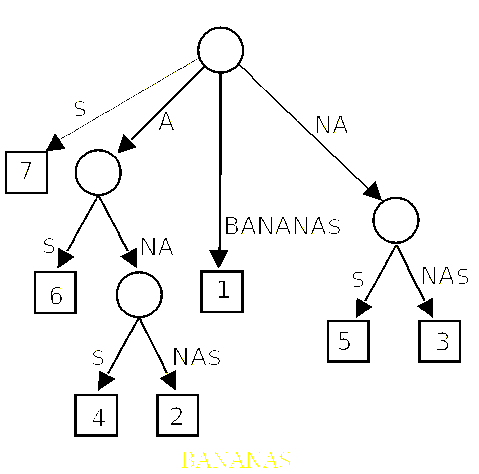
\includegraphics[scale = 0.5]{img/suf.png}
\end{center}
Una sottostringa è il \textit{prefisso di un suffisso}. Dato un
pattern voglio trovare tutti i suffissi che iniziano col
pattern. Quindi, dato che ogni nodo ha un solo figlio con un certo
prefisso, la procedura di pattern matching nel suffix-tree naviga
nell'albero sequendo il pattern nell'unico arco possibile con quel
pattern, posto che esista. Se non esiste il pattern cercato termina,
così come termina nel momento in cui lo trova raggiungendo un
$\textdollar$. Il compattamento da trie a suffix tree serve a
migliorare le performance di costruzione della struttura dati, non
quelle del pattern matching in sè. Un suffix-tree ha un rapporto tra
il numero di nodi e il numero di foglie (?).\\
Questo pattern matching ha $O(m)$ con $m$ lungheza del pattern da
ricercare ma poi ho tante foglie $k$ sotto il nodo a cui sono arrivato
quante sono le occorrenze del pattern nel testo, che quindi visito in
$O(k)$. Nel complesso ho la costruzione dell'albero in $O(n)$, $n$
lunghezza testo, matching in $O(m)$ e visita finale delle foglie in
$O(k)$, quindi nel complesso ho
\[O(n+m+k)\]
Se il pattern termina prima del passaggio ad un nodo successivo non mi
interessa in quanto i suffissi corrispondono (se ho $NA$ e mi fermo a
$N$ va bene lo stesso, in quanto i suffissi di $NA$ sono dello stesso
numero di quelli di $N$). Nelle foglie ho indicato l'indice dove
inizia ogni occorrenza.\\
Definisco la \textbf{path-label(X)} di un nodo X è la concatenazione delle
stringhe fino a quel nodo. Definisco invece \textbf{string-depth(X)} di
un nodo X la lunghezza del path-label, che è calcolabile in $O(n)$. La
string-depth di X sarà la lunghezza dell'etichetta sommata alla
string-depth del padre.\\
\textit{Molti algoritmi sfruttano molte visite per arricchire le
  informazioni dell'albero ai fini di rendere semplice la risoluzione
  di un problema.}\\
Non posso fare lo stesso ragionamento per la path-label perché,
concatendando quella del padre alla propria raggiungerei quasi
$O(n^2)$. Si usa quindi una tecnica basata su puntatori al testo e non
su stringhe, questo fa si che ogni arco sia etichettato da una coppia
di numeri (posizione di inizio e lunghezza), quindi raggiungo tempo
costante per etichettare ogni albero.\\
Il grande problema del suffix-tree è lo spazio occupato, circa $20n$
byte, quindi per il genoma umano servono 60gb di memoria. Per
risolvere questo problema si usano i \textbf{suffix array (SA)}, che occupa
meno spazio, ed è \textit{l'array dei suffissi in ordine
  lessicografico}. Il suffix array non permette il pattern matching in
tempo lineare quindi viene usato il suffix array per costruire il
suffix tree. Tutto quello che si può fare sul suffix tree si può fare
sul suffix array con tempi diversi ma simili. Non memorizzo
esplicitamente i suffissi ma memorizzo le posizioni iniziali del
suffisso. Al suffix array si aggiunge l'array ausiliario \textit{LCP
  (longest  common prefix)} con la lunghezza del prefisso comune $LPC[i]$
tra $SA[i]$ e $SA[i+1]$.
\begin{center}
  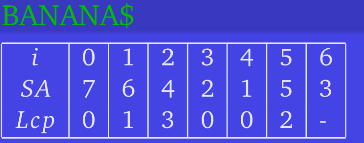
\includegraphics[scale = 0.5]{img/suf2.png}
\end{center}
Lo spazio diventa $4n$ bytes, quindi per il genoma 12gb.\\
Passiamo ora dall'albero all'array. Facciamo una visita depth-firts
(pre-order) del suffix array, assumento che a sinistra ci siano
etichette in ordine lessicografico minore (a sinistra ho suffissi con
una lettera dell'alfabeto iniziale ``precedente'').\\
Ho quindi che $LPC[i]$ è la string-depth di $LCA(i, i+1)$, ovvero
\textit{least common ancestor}, che quindi mi indica dove due percorsi
divergono e vedo quanto vale lì la string-depth.\\
Calcolare LPC costa un tempo quadratico. Ma possiamo fare un altra
cosa. Ogni arco viene visitato almeno due volte inq aundo una volta arrivati
ad una foglia si torna indietro. Mi salvo la string depth dell'LCA
nell'array ogni volta che ho un cambio di direzione nella visita dell'albero
lavorando quindi in tempo lineare. Nel disegno guardiamo due foglie
consective e contiamo i nodi che hanno in comune sopra esclusa la radice.\\
Dati SA e LCP passiamo ora a costruire l'albero. Gli LCP nulli
partizionano il SA e corrispondono ai figli della radice del suffix
array aggiungendo 1 (tre zeri corrispondono 4 figli). Di questi 4
figli prendo i valori no nulli e saranno un cammino che prosegue
ripetutamente sul valore minimo.\\
\textit{Quindi se l'array è 013002 avrò 4 figli della radice, uno 0, uno 13,
  uno 00 (che conta come 0) e uno 2. Il 13 avrà una foglia a sinistra e
  poi scenderà di un nodo. Avendo solo un numero (3) avrà due
  foglie. Infine avrò due, che essendo un solo numero, avrà solo 2
  foglie.}\\

\begin{center}
  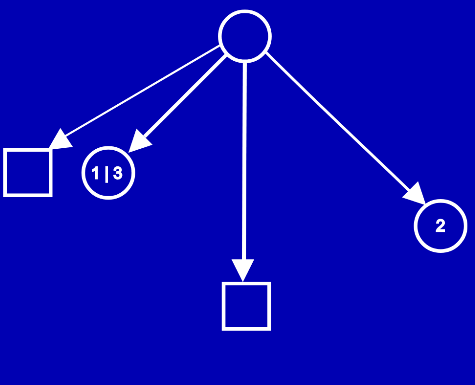
\includegraphics[scale = 0.5]{img/suf3.png}
\end{center}
\begin{center}
  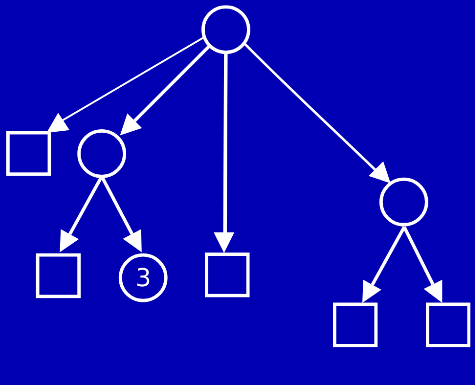
\includegraphics[scale = 0.5]{img/suf4.png}
\end{center}
\begin{center}
  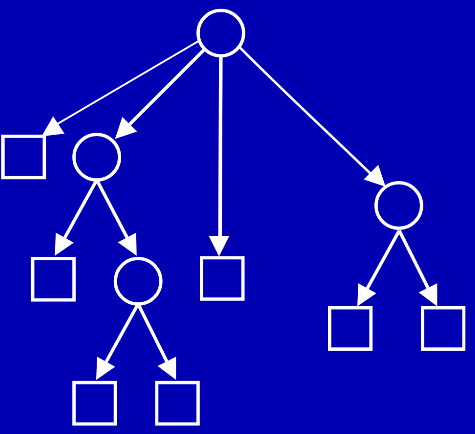
\includegraphics[scale = 0.5]{img/suf5.png}
\end{center}
\begin{center}
  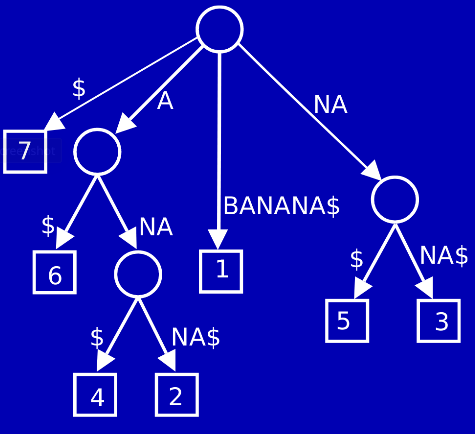
\includegraphics[scale = 0.5]{img/suf6.png}
\end{center}

Un \textbf{suffix tree generalizzato} rappresenta un insieme di
testi. Prendo x stringhe con terminatore, le concateno in un unico
testo e ne genero il suffix tree ma nelle foglie avremo le coppie
(numero stringa, posizione inizio suffisso) che potrebbero essere una
per ogni stringa e lo costruisco in tempo lineare alla lunghezza del
testo completo.
\begin{center}
  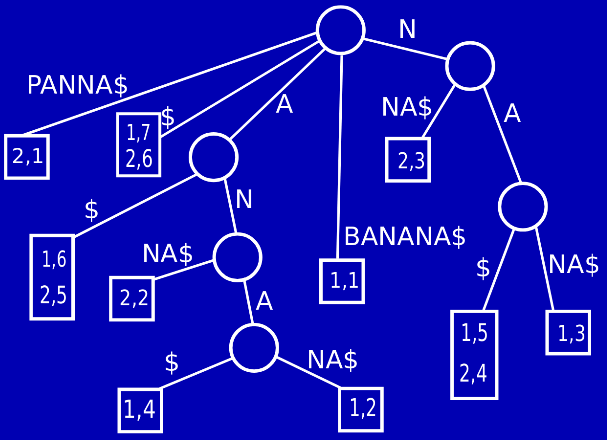
\includegraphics[scale = 0.5]{img/suf7.png}
\end{center}
Cerco ora la sottostringa comunque più lunga tra due
stringhe sfruttando il suffix tree generalizzato. Una sottostringa
comune corrisponde ad un cammino tra una radice e un nodo X e tra i
discendenti di X devo avere almeno un discendente  per ogni
stringa. La più lunga sarà quindi quella che arriva al nodo con
string-depth massimo. Visito quindi due volte l'albero, alla prima
vedo se ha le foglie giuste e la seconda per cercare il max delle
string-depth. La prima visita la faccio dalle foglie verso la radice,
creo un array di booleani per il nodo X lungo quanto il numero di
stringhe i cui elementi valgono true sse esiste un disendente di X tale che è
suffisso della stringa S. Alla fine faccio l'and tra tutti i valori
dell'array, se è true significa che ho un discendente per ogni
stringa. Se X è nodo interno faccio l'or con l'array del nodo
discendente per determinare se X va bene. Se è foglia determino il
vettore leggendone l'etichetta. La seconda visita può essere in
qualsiasi direzione e dove ho nodi con la proprietà di essere comune
alle stringhe e trovo quello con la string-depth max, ottengo quindi
un tempo che è $O(k\cdot n)$.
\subsection{Pattern Matching su Suffix Array}
Il suffix array contiene le posizioni di inizio dei suffissi ordinati
lessicograficamente e viene utilizato insieme all'LCP. Il pattern
matching in questo caso non sarà ottimale ma si
otterrà $O(m\log n)$, con $m$ lunghezza del pattern. Si sfrutta la
ricerca dicotomica, che si basa sulla ricerca a partire dall'elemento
mediano di un array, per poi cercare su una sola delle metà
dell'array, dimezzando di volta in volta l'array. La ricerca
dicotomica funziona sul suffix array ma ogni iterazione consisite nel
confrontare il pattern con i primi $m$ caratteri del suffisso mediano,
fermandosi ovviamente al primo carattere discordante per capire poi su
quale metà del suffix array continuare a cercare, basandosi sui
singoli caratteri che non matchano. Quest'ultimo passaggio è possibile
grazie al fatto che il suffix array è ordinato lessicograficamente. Si
avranno 3 aggiustamenti all'algoritmo, detti \textbf{acceleranti}, che
abbasseranno la complessità del caso pessimo (col terzo si arriva a
$O(m+\log n)$). Con gli acceleranti si evitano confronti inutili.
\\Partiamo col \textbf{primo accelerante}.\\
Si parte dal presupposto che ci sia un ordine lessicografico posso
individuare regioni, dal $L$ a $R$, in cui tutti i possibili pattern
iniziano con gli stessi caratteri iniziali.
\begin{center}
  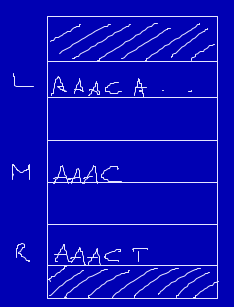
\includegraphics[scale = 0.5]{img/arr.png}
\end{center}
Formalmente si ha che tutti i fuffissi in $SA(L,R)$ iniziano con lo
stesso prefisso lungo $Lcp(SA[L], SA[R])$ e quindi potrò non
controllare i primi $Lcp(SA[L], SA[R])$ caratteri.
\\ Vediamo il \textbf{secondo accelerante}.\\
Si ha un elenco di casi che tengono in considerazione il pattern. Si
indica con $l$ l'Lcp tra il pattern e il primo suffisso
dell'intervallo e $r$ l'Lcp tra il primo e l'ultimo suffisso
dell'intervallo. Queste due variabili vengono aggiornate man mano e ho:
\begin{itemize}
  \item \textbf{caso 1:} se $l>r$ quindi il pattern somiglia più al
  primo suffisso che all'ultimo
  \begin{center}
    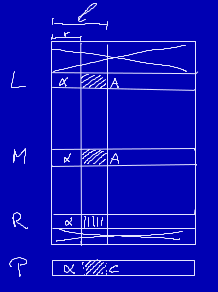
\includegraphics[scale = 0.5]{img/arr2.png}
  \end{center}
  Quindi dovrò poi controllare nella seconda metà del suffix array
  quindi scarterò in tempo costante tutta la prima metà solo se
  $Lcp(L,M)>l$, assegnando a $L$ il valore di $M$.\\
  % grafico
  Se fosse minore farei uguale scartando la seconda metà, assegnando a $R$
  il valor edi $M$ e ad $r$ l'$Lcp(M,L)$ (perché dovrò fermarmi a metà).\\
  % grafico
  Se fossero uguali dovrei confrontare $P[l+1:]$ e $M[l+1:]$ per
  decidere quale metà scartare, se avrò un carattere che non matcha
  tra il suffisso mediano e il pattern con l'ultimo carattere del
  suffisso mediano più piccolo allora cercherò nella seconda metà,
  altrimenti nella prima (sempre grazie all'ordine lessicografico).
  A differenza dei due sottocasi sopra questo
  impiega un tempo che dipende dal numero di caratteri uguali che
  trovo, più sono e più impiego tempo, anche se per assurdo più
  caratteri uguali trovo più mi sto stringendo alla regione che
  contiene il match del mio pattern. \textbf{Si ha consumo di tempo
    solo nel caso in cui mi stia avvicinando alla soluzione, se
    ``pago'' tanto in un'iterazione avrò la certezza di ``pagare''
    meno la volta seguente. Al massimo potro avere un costo pari a
    $2m$ perché ogni volta incremento o $l$ o $r$, che sommati sono
    per forza $\leq 2m$, quindi alla peggio ho complessitò $O(2m)$}.
  % grafico
  \textit{In ogni caso $l$ e $r$ potrebbero restare invariati o crescere in
    base al numero di caratteri che matchano e al massimo avranno valore
    pari alla lunghezza del pattern $m$}
  \item \textbf{caso 2:} se $l=r$. Se ho $Lcp(L,M)>l$ tengo la prima
  metà mentre se ho l'opposto   $Lcp(L,M)>l$ tengo seconda metà come
  nel primo caso.   Se invece $Lcp(L,M)=Lcp(M,R)=l$
  ragiono come nel terzo sottocaso del primo caso
  \item \textbf{caso 3:} se $l<r$ faccio lo speculare del primo caso 
\end{itemize}
\begin{esempio}
  ho i seguenti suffissi: \textit{\$, A\$, ANA\$, ANANA\$, BANANA\$,
    NA\$ e NANA\$} e pattern \textit{BA} ho quindi $L=0$, $R=6$ e $M=3$.\\
  $Lcp(L,M)=0$ e $Lcp(R,M)=0$.\\
  Confronto il primo carattere del pattern e il primo del mediano
  $B\neq A$ e $B>A$ quindi ho $L\gets 3$ mentre $R$ resta uguale (cosi
  come $r$ e $l$). Il nuovo mediano è tra 3 e 6, quindi, arrotonando,
  5.\\
  Confronto $B$ e $N$ e quindi cerco nella prima metà, che ha un solo
  elemento, quindi controllo i caratteri e scopro che, in questo caso,
  ho il match con \textit{BANANA}.
\end{esempio}
\begin{esempio}
  ho i seguenti suffissi: \textit{\$, A\$, ABRA\$, ABRACADABRA\$, ACADABRA\$,
    ADABRA\$, BRA\$, BRACADABRA\$, CADABRA\$, DABRA\$, RA\$ e
    RACADABRA\$} e pattern \textit{BRACA} ho quindi $L=0$, $R=11$ e $M=6$.\\
  $Lcp(L,M)=0$ e $Lcp(R,M)=0$.\\
  Confronto con \textit{BRA\$} e vedo che ci sono 3 caratteri uguali,
  quindi ora ho $L=6$, $R=11$, $M=9$, $l=3$ (i 3 caratteri uguali) e
  $r=0$.\\
  Confronto con \textit{DABRA\$} e vedo che il primo carattere non
  matcha e $D>B$ quindi cerco nella
  metà sopra. Quindi ora ho $L=6$, $R=9$, $M=8$, $l=3$ (i 3 caratteri uguali) e
  $r=0$.\\
  Confronto con \textit{CADABRA\$} e vedo che il primo carattere non
  matcha e $C>B$ quindi cerco nella  metà sopra.
  quindi ora ho $L=6$, $R=8$, $M=7$, $l=3$ (i 3 caratteri uguali) e
  $r=0$.\\
  Confronto con \textit{BRACADABRA\$} e vedo che ho $Lcp(L,M)=3$
  (prima era sempre stata nulla cosìccome $Lcp(R,M)$) e
  quindi sono nel terzo caso e confronto solo a partire dal terzo
  carattere escluso, trovando il match (di 5 caratteri).
\end{esempio}
Vediamo ora il \textbf{terzo accelerante (DA SISTEMARE)}.\\
Con questo accelerante studiamo il calcolo dell'Lcp. Alla prima
iterazione avrò $L=1$ e $R=n$, alla seconda avrò o $L=1$ e
$=\frac{n}{2}$ oppure $L=\frac{n}{2}$ e $R=n$ (a seconda della metà
scelta). Ad interazione $k$ avrò una forma del tipo $L=h\frac{n}{2^{k-1}}$ e
$R=(h+1)\frac{n}{2^{k-1}}$ con $h$ che rappresenta l'indice
dell'intervallo (al primo giro ho $h=\{1,2\}$, al secondo in
$h=\{1,2,3,4\}$ $\ldots$ $h=\{1,\ldots, 2^{k}\}$). Al termine
della mia ricerca dicotimica ho intervalli di cardinalità due. Sempre
alla fine della ricerca dicotomica si avranno al massimo $n$
intervalli. Entra quindi in gioco il terzo accelerante, che consiste
nel preprocessare tutti gli intervalli, quindi precalcola tutti i vari
Lcp. \textbf{Questo accelerante è di solo interesse teorico}. Voglio
calcolare abbastanza velocemente questi Lcp. Per ogni intervallo
calcolo l'Lcp ma in realtà per intervalli consecutivi (quindi nel caso
k-simo) ho già l'array Lcp e per ottenere gli altri aggrego i
risultati dell'interazione. Quindi Lcp tra un $L$ e un $R$ è il minimo
tra l'Lcp della prima metà, l'Lcp della seconda meta e l'Lcp tra $M$ e
$M+1$ che è nell'array Lcp (mentre quelli delle due metà sono già
calcolate).
% aggiungo formula
Ottengo quindi un $O(n)$.\\
Ho quindi ottenuto l'algoritmo per trovare un'occorrenza, che non è
per forza la prima. Voglio ora espandere per trovare tutte le
occorrenze in un tempo proprorzionale al numero stesso di
occorrenze. So che tutte le occorenze sono in un intorno
dell'occorrenza trovata. Cerco quindi i suffisi precedente e seguenti
fino a non trovare alcun match. Parto con l'occorrenza precedente e
uso l'array Lcp, in quanto controllo suffissi consecutivi, con l'array
vedo quanti caratteri iniziali condidono e se ne condividono almeno
$m$ (cardinalità del pattern) allora ho trovato un'altra
occorrenza. Dovendo solo leggere un valore ho tempo costante e quindi
nel complesso ho un $O(n+m+k)$ con $k$ numero di occorrenze.\\
In totale calcolo suffix array, array Lcp, preprocessamento e
scansione per trovare tutte le occorrenze, il tutto in $O(m\log n)$
\subsubsection{Pattern Matching}
Per calcolare la sottostringa comune più lunga ho i seguenti step:
\begin{enumerate}
  \item calcolo il suffix tree generalizzato della stringa $S$
  \item cerco il nodo $x$ tale che:
  \begin{enumerate}
    \item per ogni stringa $s_i \in S$ esiste un discendente di $x$
    corrispondente ad un suffisso di una delle stringhe $s_i$
    \item abbia la string-depth di massima fra tutti i nodi con la
    stessa caratteristica
  \end{enumerate}
\end{enumerate}
Dobbiamo ``rimappare'' questo ragionamento sul suffix array.\\
Una volta che i suffissi sono ordinati lessicograficamente essi
appaiono consecutivamente nel suffix tree (di $n$ nodi), come se
fossero una porzione contigua del suffix array. Però dal suffix array
posso estrarre $n\choose 2$ intervalli.\\
Parto quindi da un suffix array generalizzato (col suo array
LCP). Estraggo un generico intervallo $[i:j]$ del suffix array,
provando ad estrarli tutti, mi salvo il prefisso comune $p$ di tutti i
suffissi in quell'intervallo e se quell'intervallo contiene almeno un
suffisso per ogni stringa $s_i\in S$ e la lunghezza del prefisso
estratto $p$ è maggiore di $t$ (maggior lunghezza fino a quel momento)
allora mi salvo quella $p$ in $t$. Ma questa tecnica non può essere
lineare. Posso quindi diminuire il numero di intervalli da considerare
e devo calcolare velocemente la lunghezza del prefisso comune in $p$
(nel tree era facile calcolarlo in quanto si usava la string-depth).\\
Iniziamo col vedere come ridurre gli intervalli, cercando quelli
inutili. Fissato un punto finale $j$ guardo tutti gli intervalli che
finisono in $j$. Per ogni $j$ che controllo voglio considerare solo un
punto di inizio $i$. Non voglio intervalli con suffissi di una sola
della stringhe in ingresso. Presi un $l\leq i \leq j \leq q$ e
considero il $SA[i:j]$ e $SA[l:q]$ con il primo intervallo quindi
incluso nel secondo. Se $SA[l:q]$ non contiene nemmeno un suffisso per ogni
stringa in ingresso allora anche $SA[i:j]$ farà lo stesso. Sia quindi
$t_1$ un prefisso comune di $SA[i:j]$ e $t_2$ di $SA[l:q]$ allora la
lunghezza di $t_1$ è $\geq$ di quella di $t_2$. Cerco quindi l'unico
punto di inizio per ogni fine $j$ che ha senso considerare, ovvero
calcolo il massimo $i$ tale per cui $SA[i:j]$ contiene almeno un
suffisso per ogni stringa in ingresso, ho quindi un numero lineare di
intervalli da considerare. Per calcolare $i$ tengo traccia, per ogni
stringa in ingresso, di ogni ultima volta che ho un suffisso (creo
quindi un array $last$). Fissato $j$ quindi prendo l'intervallo minimo
che finisce in $j$ e sfrutto l'array $last$. Quindi $i$ sarà il
massimo valore tale che $SA[i:j]$ contiene almeno un suffisso per ogni
stringa in ingresso.
\textbf{capire}
% aggiungere disegno
Quindi considero un intervallo $[i:j]$ e la lunghezza del
prefisso comune a tutti i suffissi che è uguale al minimo dell'LCP tra
$i$ e $j-1$\\
Questo sistema comporta un tempo quadratico e bisogna arrivare ad un
tempo lineare.\\
Io ho un array $A$ di $n$ elementi e voglio calcolare il minimo in un
certo intervallo. È il \textbf{range minimun query}. Vogliamo
indicizzare in tempo $O(n\log n)$ e calcoleremo, grazie a questo
preprocessamento, il minimo in di un intervallo in tempo costante
$O(1)$. Il sistema consiste nel precalcolare i minimi per alcuni
intervalli che bastano per tutti. Il calcolo del minimo sarà poi un
confronto tra due intervalli. Se voglio il minimo in un intervallo e
ho precalcolato il minimo di due intervalli che insieme coprono
l'intero intervallo allora mi basta confrontare i due minimi dei
sottointervalli pre calcolati. \\
Preprocesso quindi piccoli intervalli ma che nel complesso mi coprano,
a coppie, tutto l'intervallo completo. Partiamo cercando un $z$ tale
che $2^z\leq j-i+1$ e prendo poi due intervalli, uno $[i:i+2^z-1]$ e
uno $[j-2^z+1:j]$. Ho quindi che $z=\left\lfloor{\log_2
    j-i+1}\right\rfloor$. Uso quindi la programmazione dinamica con
una matrice $B[x,y]=\min_{x\leq z<x+2^{y}}A[z]$:
\[
  \begin{cases}
    B[x,0]=A[x]\\
    B[x,y]=\min\{B[x,y-1], B[x+2^{y-1},y-1]\} \mbox { se } y\geq 0\\
  \end{cases}
\]
nel complesso ho quindi $n\log n$ elementi. Costruita questa matrice
vado a prendere il:
\[\min\{B[i,wr],B[j-2^w+1,w]\}\]
dove $w$ è la più grande potenza di 2 minore o uguale a $j-i+1$.
\textbf{finire}\\
\chapter{Allineamenti}
Ovviamente in bioinformatica uno dei problemi principali è il
confronto di sequenze biologiche per lo studio, per esempio, delle
proteine, alla ricerca di similitudini tra sequenze. Una sequenza
biologica si basa su un alfaberto formato dalle basi azotate:
\[\Sigma=\{A,C,T,G\}\]
In biologia molecolare si ha che \textbf{se due sequenze sono
  strutturalmente simili allora hanno anche una funzione simile}.
Si ha quindi la \textit{ricerca di omologie}, anche per lo studio
dell'evoluzione.
\begin{definizione}
  Si definsice \textbf{distanza di Hamming} il numero totale di
  caratteri differenti, a parità di posizione, tra due stringhe:
  \[d:S\times S\to\mathbb{R}^+\]
  con $S\times S$ insieme delle coppie di stringhe.\\
  La distanza di Hamming gode di:
  \begin{itemize}
    \item \textbf{riflessività}: $d(x,y)=0\Longleftrightarrow x=y,\,\,\forall
    x,y\in S$
    \item \textbf{simmetria}: $d(x,y)=d(y,x),\,\,\,\forall
    x,y\in S$
    \item \textbf{diseguaglianza triangolare}: $d(x,y)+d(y,z)\leq
    d(x,z),\,\,\,\forall x,y\in S$
  \end{itemize}
  \textbf{La distanza di Hamming è definita unicamente per stringhe di
  egual lunghezza}
\end{definizione}
\section{Allineamento globale}
Si analizza l'allineamento di due intere stringhe, si ha quindi un
problema di \textbf{ottimo gloable}. Si analizzano due stringhe di
lunghezza arbitraria e non uguale tra di loro. Ci si riconduce all'uso
della distanza di Hamming inserendo spazi fino ad ottenere due
stringhe di egual lunghezza per poter lavorare colonna per colonna.
Si usano caratteri \textbf{indel} (\textit{in} inserisco e
\textit{del} tolgo). Si hanno delle proprietà:
\begin{itemize}
  \item non si possono avere colonne di soli indel
  \item le stringhe estese con gli indel devono essere lunghe uguali
\end{itemize}
Per esempio si ha quindi:
\begin{center}
  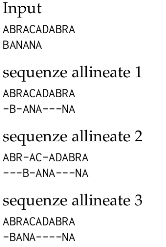
\includegraphics[scale = 0.7]{img/indel.png}
\end{center}
Un buon allineamento deve contenere pochi indel, molti caratteri
allineati e pochi non allineati.\\
\begin{definizione}
  Un problema di ottimizzazione richiede:
  \begin{itemize}
    \item un'istanza che è un insieme infinito di casi
    \item un insieme di soluzioni ammissibili verificabili in tempo
    polinomiale
    \item una funzione obiettivo, che è una soluzione ammissibile che
    mappa in $\mathbb{Q}$
    \item una soluzione che massimizza (massimizza il valore) o
    minimizza (minimizza il costo) la funzione obiettivo
  \end{itemize}
\end{definizione}
Si usa quindi la programmazione dinamica per stabilire uno score che
cresce quando i valori delle colonne coincidono e quindi si cerca di
massimizzare questo valore.\\
Cerchiamo quindi l'equazione di ricorrenza di questo problema di
massimizzazione.\\
Innazitutto abbiamo come variabile una matrice di score:
\[d:\left(\Sigma\cup\{-\}\right)\times\left\(\Sigma\cup
    \{-\}\right)\to \mathbb{Q}\]
Quindi date due stringhe $s_1$ e $s_2$ si ha che:
\[M[i,j]=\mbox{ottimo su} s_1[:i],\,s_2[:j]\]
con la seguente equazione di ricorrenza, detta di
\textbf{Needleman-Wunsch} (si indicano con ``-'' gli indel):
\[M[i,j]=\max
  \begin{cases}
    M[i-1,j-1]+d(s_1[i],s_2[j]) & \mbox{se non ho indel}\\
    M[i,j-1]+d(-,s_2[j]) & \mbox{se ho indel solo in }s_1\\
    M[i-1,j]+d(s_1[i],-) & \mbox{se ho indel solo in }s_2
  \end{cases}
\]
con le seguenti condizioni a contorno:
\[
  \begin{cases}
    M[0,0]=0\\
    M[i,0]=M[i-1,0]+d(-,s_2[j])\\
    M[0,j]=M[0,j-1]+d(-,s_2[j])
  \end{cases}
\]
Si ha quindi un doppio ciclo for e un tempo pari a $O(nm)$.\\
Fino ad ora si è aprlato di \textbf{allineamento globale}. Si
definisce invece \textbf{allineamento locale} l'individuazione di due
sottostringhe $t_1\subseteq s_1$ e $t_2\subseteq s_2$. Date altre due
sottostringhe $u_1,u_2$ delle 2 stringhe si ha che:
\[M[t_1,t_2]\geq M[u_1,u_2]\]
Un algoritmo banale avrebbe tempi assurdi: $O(n^3m^3)$.\\
Questo problema si può risolvere velocemente con il metodo
\textbf{Smith-Waterman}.\\
Con questo metodo l'allineamento viene ricercato tra tutte le
sottostribghe terminanti nelle posizioni $i$ e $j$, ovvero
$t_1=s_1[h,i]$ e $t_2=s_2[k,j]$, con $h$ e $k$ incogniti e con massimo
valore di $M[t_1,t_2]$. Si richiede inoltre che l'allineamento
ottimo abbia un'ultima colonna senza indel. Grazie a questa clausola
si ha che $s_1[h,i-1]$ e $s_2[h,j-1]$ è l'allineamento ottimale delle
sottostrighe terminanti un carattere prima di $i$ e $j$. Supponiamo
che queste ultime due sottostringhe inizino da $a$ e $b$ e che:
\[M(s_1[a,i-1],s_2[b,j-1])>M(s_1[h,i-1],s_2[k,j-1])\]
Aggiungiamo ora anche la colonna $i$ e quella $j$. Se si hanno
caratteri uguali nell'ultima colonna si ha che:
\[M(s_1[a,i],s_2[b,j])>M(s_1[h,i],s_2[k,j])\]
Ma questo è un assurdo essendo $M(s_1[h,i],s_2[k,j]$ massimo per
ipotesi.\\
Questo ragionamento si estende anche ai casi in cui ci sia un'indel a
termine di una delle due stringhe. Si introduce anche un nuovo caso,
aggiuntivo rispetto a quelli di Needleman-Wunsch: il caso in cui
nessuna sottostringa ha un allineamento positivo. In questo caso se
precedentemente non ci sono match si setta la casella a 0 e si evitano
i valori negativi. Una conseguenza diretta è che:
\[M[0,0]=M[i,0]=M[0,j]=0\]
Dopo aver costruito la matrice cerco il valore massimo e le coordinate
$x,y$ indicano le posizioni finali delle sottostringhe mentre le
coordinate del primo 0 indicano le posizioni iniziali.\\
Definiamo quindi l'equazione di ricorrenza:
\[M[i,j]=\max
  \begin{cases}
    M[i-1,j-1]+d(s_1[i],s_2[j]) & \mbox{se non ho indel}\\
    M[i,j-1]+d(-,s_2[j]) & \mbox{se ho indel solo in }s_1\\
    M[i-1,j]+d(s_1[i],-) & \mbox{se ho indel solo in }s_2\\
    0 & \mbox{altrimenti}
  \end{cases}
\]
Si è quindi raggiunto un $O(nm)$.\\
Graficamente si ha:
\begin{center}
  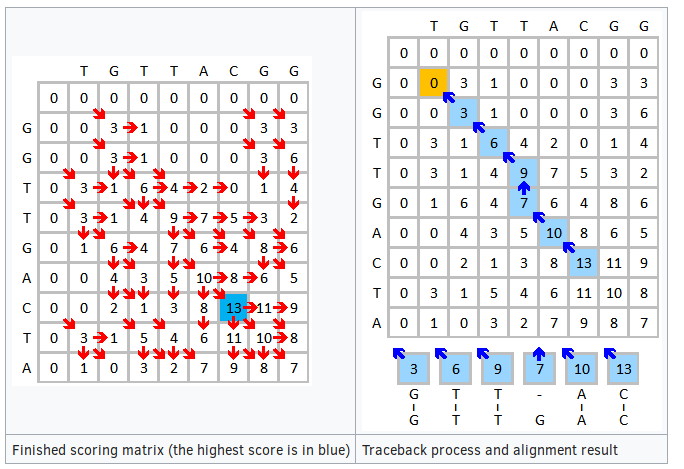
\includegraphics[scale = 0.5]{img/sw.png}
\end{center}
\begin{definizione}
  La \textbf{distanza di Edit} è la trasformazione di una stringa in
  un'altra tramite l'inserimento, la cacncellazione o la modifica di
  un carattere. Inoltre si ha che la distanza di edit è un caso
  particolare dell'allineamento globale tra due sequenze.\\
  \textbf{L'allineamento globale racchiude tutte le possibili
    casistiche delle distenze di Edit}.\\
  Si ha la seguente equazione di ricorrenza:
  \[M[i,j]=\min
    \begin{cases}
      M[i-1,j-1] & \mbox{se } s_1[i]=s_2[j]\\
      M[i-1,j] & \mbox{se viene cancellato un carattere}\\
      M[i,j-1] & \mbox{se viene aggiunto un carattere}\\
      M[i-1,j-1]+1 & \mbox{se viene modificato un carattere}
    \end{cases}
  \]
\end{definizione}
Sulla stringa si procede da sinistra a destra.\\
Quindi il costo di ogni mismatch è pari a 1. \\
La distanza di Edit ha tempo $O(nm)$
\textbf{rivedere completamente}
\begin{shaded}
  Con LCS abbiamo un problema di massimizzazione dove mettiamo nella
  matrice di score 1 in corrispondenza di caratteri uguali e 0 negli
  altri casi. Con la distanza di Edit abbiamo 0 in caso di uguali
  caratteri e 1 nelle altre posizioni. Le due matrici di score sono
  quindi complementari. 
\end{shaded}
Facciamo un altro ragionamento. Penso ad un allineamento di minimo
costo dove ``taglio'' un prefisso e un suffisso delle due stringhe,
ovviamente un prefisso o un suffisso di una delle due stringhe.
Quindi, dato che parliamo di minimizzazione, quanto taglio ha
costo 0. Bisogna trovare un modo per imporre costo 0 per i caratteri
scartati ragionando sull'equazione di ricorrenza \textbf{senza toccare la
  matrice di score}. Basta modificare le condizioni a contorno,
mettendo a 0 la prima riga e la prima colonna:
\[
  \begin{cases}
    M[0,0]=0\\
    M[i,0]=0\\
    M[0,j]=0
  \end{cases}
\]
\textbf{Abbiamo quindi una nuova variante dell'allineamento globale
  dove minimizziamo il costo e non massimiziamo la validità, scartando
  un prefisso di una delle due stringhe}.\\
\textit{Questo proedimento è comodo se si hanno stringhe di lunghezza
  molto diversa, trovando un allineamento buono in modo che dove si
  allineano si abbiano pochi indel}.\\
Abbiamo visto come scartare un prefisso, ora ragioniamo sul suffisso.
Cerco quindi il minimo nell'ultima riga e nell'ultima colonna e
decido di conseguenza quale suffisso scartare e i quale stringa (se è
nell'ultima riga scarto da $s_2$, se nella colonna è in $s_1$).\\
Un altra variante prevede una lunghezza $k$ del prefisso o suffisso
da scartare. Per il suffisso ragiono solo le ultime $k$ posizioni
nell'ultima riga e dell'ultima colonna, mentre per il prefisso metto 0
solo nelle prime k posizioni della prima riga e della prima colonna.\\
In ogni caso per ricorstruire risalgo fino ad un 0.\\
Analizziamo un ulteriore approccio. Questa volta si è interessati solo
al costo di un allineamento globale, cercando però di ottimizzare
sullo spazio. Per calcolare $M[i,j]$, essendo una LCS, mi bastano solo
il valore a sinistra $M[i-1,j]$, quello sopra $M[i,j-1]$ e quello
precedente sulla diagonale $M[i-1,j-1]$. Quindi mi basta tenere la
riga o la colonna in cui sono e la riga o la colonna precedente,
scegliendo la riga o la  colonna in base alla loro lunghezza, che
corrisponde quindi alla lunghezza della stringa (se $s_2$ è più corta
scelgo la riga altrimenti, se $s_1$ è più corta, la colonna). Non
serve quindi tenere tutta la matrice e posso quindi risparmiare
spazio.\\
Ora restringiamo ancora l'allineamento, cercando di risolvere
l'allineamento su stringhe molto simili, in maniera ancora più
ottimizzata sfruttando la similarità. In altre parole si ha la
distanza di Edit con un numero di operazioni che è al massimo un
valore $k$, tutto in $O(kn)$. Voglio ridurre il tempo di calcolo dela
distanza di Edit sapendo che vale al massimo $k$. Avrò quindi al
massimo $kn$ caselle.\\
Sapendo che ho la distanza di Edit tra le due stringhe  vale al
massimo $k$ e che le due stringhe sono lunghe $n$ e $m$ so che:
\[|n-m|\leq k\]
Si ha quindi una matrice di programmazione dinamica che è quasi
quadrata. Si ha che le parti che non costano corrispondono ad uno
spostamento sulla diagonale, quindi al diminuire della distanza di
Edit mi avvicino alla diagonale principale. Posso quindi non
considerare le caselle lontane della diagonale. È l'\textbf{allineamento
  mediante distanza di Edit con banda}, ovvero seleziono un intorno
della diagonale principale (appunto una banda) da analizzare, perché
fuori dalla stessa avrò solo soluzioni non ottimali.\\
\textbf{disegno}\\
Si arricchiscono ancora le condizioni a contorno della ricorrenza
della distanza di Edit, ponendo a $-\infty$ le caselle in cui
$|i-j|\geq k$ (nel codice si avrebbe solo questo controllo).
Si potrebbe però non conoscere $k$ o si potrebbe avere un $k$
sbagliato, portando ad una soluzione non ottima (magari perché questa
soluzione vorebbe ``uscire'' nell'area fuori dalla banda). Si procede
quindi raddoppiando $k$ e mi fermo quando la distanza di Edit $edit$ è,
per un certo $h$ che alla fine varrà $h^*=\log_2 edit$:
\[2^{h-1}<edit<2^h\]
Ho quindi tempo complessivo pari a:
\[\sum_{i=0}^{h^*}O(2^in)=O(n)\cdot\sum_{i=0}^{h^*}O(2^i)=O(n)\cdot
  (2^{h^*+1}-1)\sim O(n)\cdot (2^{h^*}-1)\]
\[\Downarrow\]
\[O(n)\cdot (2\cdot edit -1)=O(n\cdot edit)\]
Abbiamo quindi un buon tempo, rispetto a $O(nm)$.\\
\textit{Si raddoppia per essere comodi coi conti con il logaritmo.}\\
\textbf{Ovviamente questa strategia funziona bene sse le stringhe sono
  abbastanza simili, con $k<<n$ e $k<<m$.}\\
Vediamo un'altra variante di allineamento. Ogni volta che si
introducono indel si ha un forte ``significato'' biologico. Quando si
aggiunge un indel si sposta il frame di lettura e si shiftano di uno i
codoni. 
\begin{definizione}
  Si definisce \textbf{gap} una sequenza contigua di indel
\end{definizione}
Si ha che tra inserire un indel e un gap si ha poca differenza. Si ha
quindi che ogni gap è associato ad un costo legato alla sua lunghezza
$P(l)$. Per l'allineamento separo quindi in match e mismatch tra
caratteri e in costi in presenza di gap.\\
Si vuole ottenere che allungare di uno un gap deve avere costo
costante (allungare un gap da 1 a 2 deve costare come da 11 a 12).\\
L'ultima colonna dell'allineamento ottimo quindi varia rispetto a
quella standard dell'allineamento globale.\\
Quindi $M[i,j]$ è l'allineameno ottimo si $s_i[1:]$ e $s_2[:j]$.\\
Cerco quindi la mia equazione di ricorrenza dove si devono considerare
i gap. Ma non posso scrivere un'unica equazione di ricorrenza che
consideri tutte le possibili lunghezze dei gap. Cerco quindi l'ultima
componente per la matrice della programmazione dinamica, che sono
l'ultima colonna in assenza di gap o la posizione dell'ultimo
gap. Ottengo quindi:
\[M[i,j]=\max
  \begin{cases}
    M[i-1,j-1]+d(s_i[i],s_2[j]) & \mbox{se non ho gap} \\
    \max_{l>0} M[i,j-l]+P(l) & \mbox{se ho gap in }$s_1$ \\
    \max_{l>0} M[i-l,j]+P(l) & \mbox{se ho gap in }$s_2$
  \end{cases}
\]
Ponendo come condizione a contorno che:
\[M[0,0]=0\]
\[M[i,0]=P(i)\]
\[M[0,j]=P(j)\]
Per i tempi ho, con un'analisi iniziale grezza, sapendo che riempire
una casella costa $i+j+1$:
\[\sum_{i=0}^n\sum_{j=0}^m(i+j)\leq nm(n+m)=n^2m+nm^2\]
E non si può scendere sotto questo caso pessimo. Ipotizziamo di
dividere in 4 la matrice, del quadrante in basso a destra ho $i\geq
\frac{n}{2}$ e $j\geq\frac{m}{2}$ e quindi ho
\[t\geq \frac{nm}{4}\left(\frac{n}{2}+\frac{m}{2}\right)\geq
  \frac{1}{8}nm(n+m)\]
tutto questo solo nell'ultimo quadrante. È quindi impossibile scendere
sotto quel caso pessimo. \textbf{Questo, $O(nm(n+m))$, è il ``prezzo
  da pagare'' per avere costo di gap generico, dove un gap lungo $n$
  costa meno di $n$ gaps lunghi 1}.\\
Bisogna quindi cambiare approccio per migliorare l'algoritmo,
riducendo i valori da calcolare, in quanto ora leggo tutti i valori
sopra, tutti quelli a sinistra e quello precedente sulla diagonale. Si
passa al \textbf{gap affine o lineare}, dove si ha una penalità $P_o$
di apertura del gap più $l$ volte quella di estenione del gap $P_e$:
\[costo=P_o+l\cdot P_e,\,\,\,P_e,P_o<0\]
Quindi la creazione costa un valore che tiene conto di $P_o$ e $P_e$
mentre l'aumento del gap varia solo su $P_e$. Vista questa situazione
cerco le casistiche dell'ultima componente da guardare. Alla
situazione di prima si aggiungono dei casi. Si cerca l'allineamento
ottimo di $s_1[i-1]$ e $s_2[j:]$ sotto la condizione che l'ultima
colonna di tale allineamento abbia un indel per $s_2$ (e si cerca
anche il problema simmetrico a questo per $s_1$). Si hanno quindi
ottimi vincolati.
\newpage
Si ha quindi: 
\[M[i,j]=\mbox{ ottimo su } s_1[:i],\,s_2[:j]\]
\[E_1[i,j]=\mbox{ ottimo su } s_1[:i],\,s_2[:j] \mbox{ con estensione
    di gap finale in }s_1\]
\[E_2[i,j]=\mbox{ ottimo su } s_1[:i],\,s_2[:j] \mbox{ con estensione
    di gap finale in }s_1\]
\[E_1[i,j]=\mbox{ ottimo su } s_1[:i],\,s_2[:j] \mbox{ con apertura
    di gap alla fine di }s_1\]
\[N_2[i,j]=\mbox{ ottimo su } s_1[:i],\,s_2[:j] \mbox{  con apertura
    di gap alla fine di }s_2\]
quindi:
\[M[i,j]=\max
  \begin{cases}
    M[i-1,j-1]+d(s_1[i],s_2[j])\\
    E_1[i,j],E_2[i,j]\\
    N_1[i,j],N_2[i,j]
  \end{cases}
\]
\[E_1[i,j]=\max
  \begin{cases}
    E_1[i,j-1]+P_e\\
    N_1[i,j-1]+P_e
  \end{cases}
\]
\[E_2[i,j]=\max
  \begin{cases}
    E_2[i-1,j]+P_e\\
    N_2[i-1,j]+P_e
  \end{cases}
\]
\[N_1[i,j]=M[i,j-1]+P_o+P_e\]
\[N_2[i,j]=M[i-1,j]+P_o+P_e\]
Si ha quindi tempo costante per ogni casella e ottengo tempo pari a
$O(nm)$ anche se ho una costante superiore (5) che moltiplica $nm$ da
considerare i termini di spazio.\\
\textit{Si può volendo compattare in 3 matrici.}\\
\textbf{Ho programmazione dinamica in termini di soluzioni di
  sottoistanze ottime di altri problemi collegati al primo}\\
\subsection{Allineamento multiplo}

\end{document}
